%
% Unless otherwise indicated, the copyright in this material is 
% owned by Joerg Evermann. This material is licensed to you under the 
% Creative Commons by-attribution non-commercial license (CC BY-NC 4.0)}
%

\section*{Sources and Further Reading}

The material in this chapter is based on the following sources. They are freely available. Consult them for additional information.

\begin{tcolorbox}[colback=alert]
Gareth James, Daniel Witten, Trevor Hastie and Robert Tibshirani: \emph{An Introduction to Statistical Learning with Applications in R}. 2nd edition, corrected printing, June 2023. (ISLR2) \\
\vspace{1mm}
\url{https://www.statlearning.com} \\
\vspace{1mm}
Chapter 12
\end{tcolorbox}

The book by James et al. provides an easy introduction to machine learning at the introductory undergraduate level. It focuses on applications, not mathematics, and contains many exercises using R. Concepts are well explained and illustrated. There is a similar book available by the same authors with applications in Python. This book is a more accessible of the following book.

\begin{tcolorbox}[colback=alert]
Trevor Hastie, Robert Tibshirani, and Jerome Friedman: \emph{The Elements of Statistical Learning}. 2nd edition, 12th corrected printing, 2017. (ESL) \\
\vspace{1mm}
\url{https://hastie.su.domains/ElemStatLearn/} \\
\vspace{1mm}
Chapter 14
\end{tcolorbox}

The book by Hastie et al. still sets the standard for statistical learning. It is widely used and cited. It's treatment is more technical than the previous book and there are no exercises in R or Python. However, it covers the concepts in more depth (and a few more formulas). However, it is still very accessible even to an undergraduate audience.

\begin{tcolorbox}[colback=alert]
Kevin P. Murphy: \emph{Probabilistic Machine Learning -- An Introduction}. MIT Press 2022. \\
\vspace{1mm}
\url{https://probml.github.io/pml-book/book1.html} \\
\vspace{1mm}
Chapters 20, 21
\end{tcolorbox}

Murphy's book is available under a creative-commons license. It is a somewhat more technical treatment of the material, but with many illustrations and examples. It is quite comprehensive in its coverage and targeted at the advanced undergraduate or graduate student. 

\section{Introduction}

In unsupervised machine learning, there are no known correct outputs that can be used to train or fit statistical models. In that sense, there are no $X$ and $Y$ variables, but only the $X$ variables. Unsupervised machine learning focuses on identifying patterns in the data, often in order to simplify the data. The two unsupervised methods considered here, principal components analysis (PCA) and cluster analysis or clustering, both do this. For example, PCA ''summarizes'' multiple variables or ''dimensions'' into fewer variables, the principal components, while cluster analysis finds similarities in the data and groups or clusters observations into fewer clusters than observations. The principal components and the clusters can be viewed as simpliciations or summaries of the data. 

\section{Principal Components Analysis}

The aim of \emph{principal component analysis} (PCA) is to create linear combinations of the input variables, the principal components (PC), that satisfy two conditions:

\begin{enumerate}
\item They are maximally variable, that is, their variance is maximal, and
\item They are orthogonal, that is, independent, of each other.
\end{enumerate}

There are as many principal components as there are input variables. Generally, only a few of the principal components, the ones with the greatest variance, are retained for further analysis. It is not uncommon to reduce hundreds of variables to five or ten principal components for further analysis.

These principal components are considered summaries of the original data and can be used, for example, instead of the original input variables in a regression or classification model. This makes the model smaller and therefore easier to understand, interpret, and verify. Using fewer inputs for a regression or classification can also serve as a regularization method, that is, a way to make the model less susceptible to overfitting. This is because models with fewer inputs generally have fewer parameters, all other things being equal. Additionally, the principal components are useful for data visualization. It is much easier to show a 2D or 3D summary of the data when the data has been summarized in two or three principal components, rather than visually depicting dozens or hundreds of variables. 

Figure~\ref{fig:pca1} shows an example visualization of a scatterplot of data on two variables and the two principal components. Technically, the two arrows shown are the \emph{eigenvectors} of the covariance matrix of the data, scaled in length by the square root of the corresponding \emph{eigenvalue} and then shifted to the mean of the data, details that will become clear below.

\begin{figure}
\centering
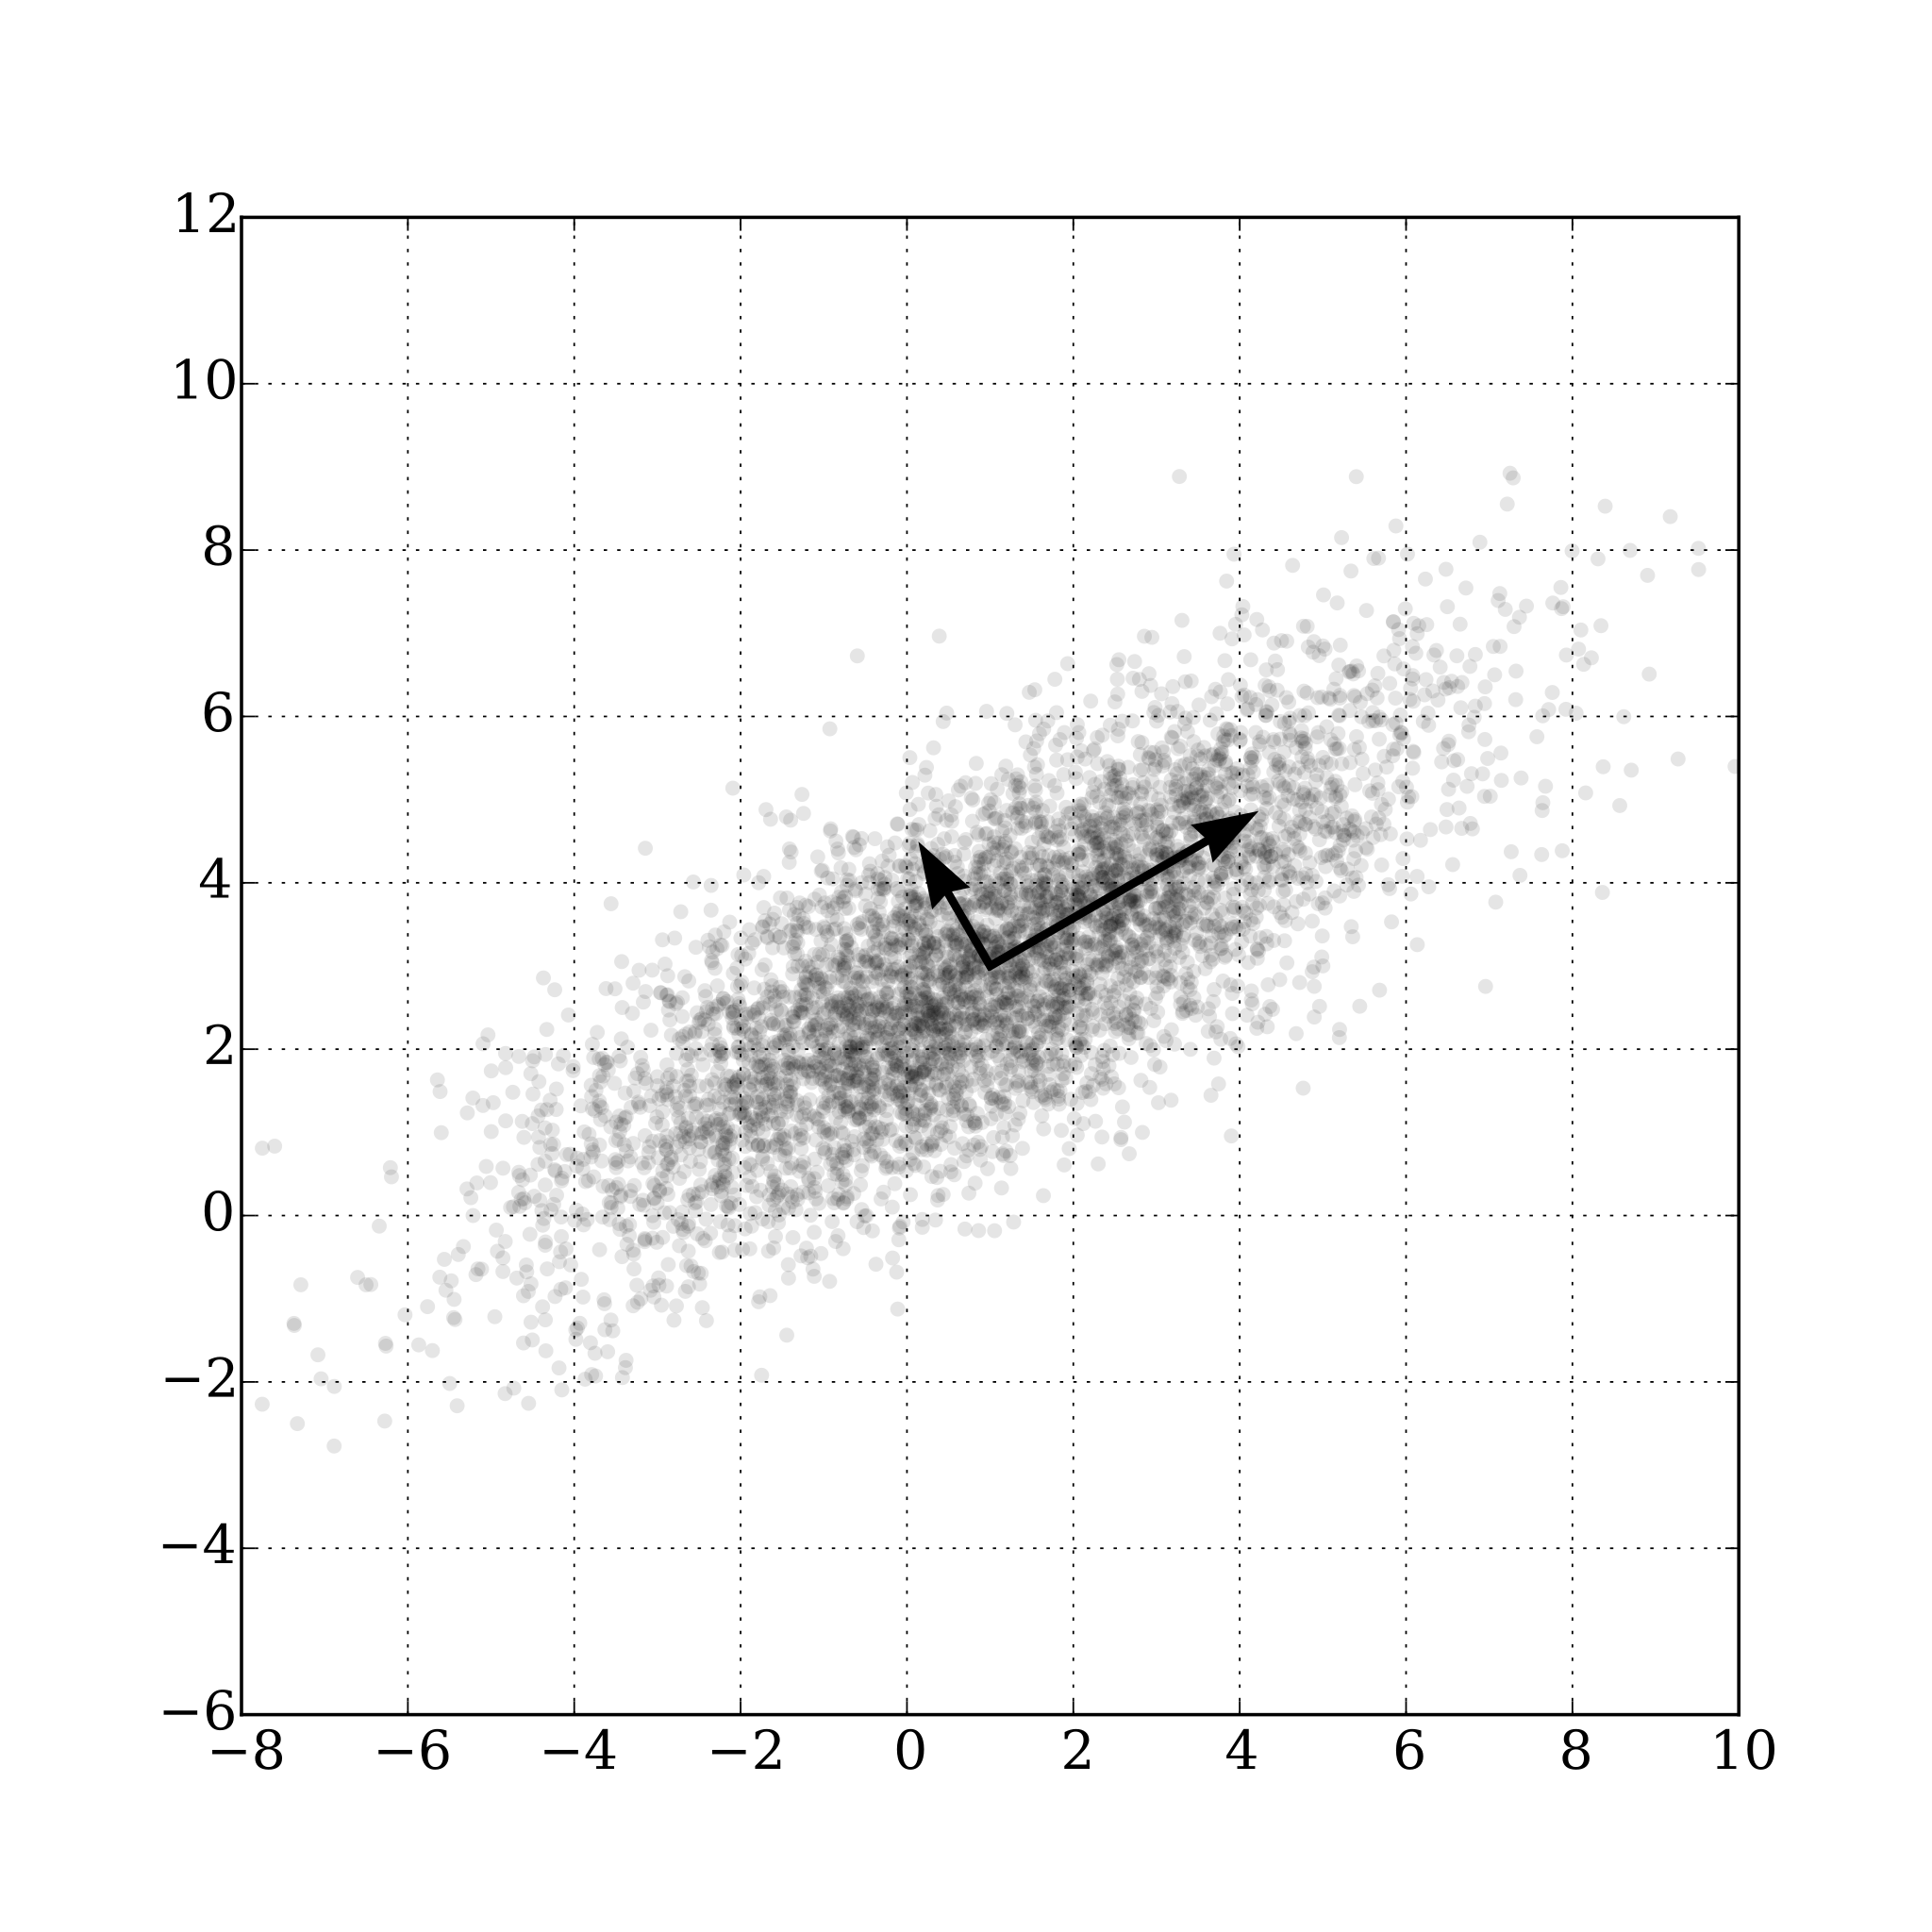
\includegraphics[width=.75\textwidth]{GaussianScatterPCA.svg.png} \\
\scriptsize
\url{https://commons.wikimedia.org/wiki/File:GaussianScatterPCA.svg} \\
\caption{Scatterplot with Principal Components}
\label{fig:pca1}
\end{figure}

We first introduce an iterative method of computing principal components. Recall that principal components are linear combinations of the original input variables. Hence, the first principal component (PC) for $1 \leq i \leq n$ data values and $p$ variables is defined as:
\begin{align*}
z_{i1} &= w_{11} x_{i1} + w_{21} x_{i2} + \cdots + w_{p1} x_{ip}
\end{align*}
Or, simpler, in matrix form:
\begin{align*}
Z_1 = X w_1
\end{align*}

\noindent The \emph{weight vector} or \emph{loading vector} $w_1 = (w_{11}, \ldots , w_{p1})$ is a $p \times 1$ column vector that is scaled to unit length, that is, $||w_1||_2 = 1$. $X$ is a $n \times p$ data matrix and $Z_1$ is the first principal component of size $n \times 1$. 

Assuming zero-centered variables, the variance of $Z_1$ and the optimization criterion can be expressed as follows:

\begin{align}
\operatorname*{maximize}_{w_{j1}} \; \sum_{i=1}^n z_{i1}^2 = \sum_{i=1}^n \left( \sum_{j=1}^p w_{j1}x_{ij} \right)^2 \qquad \text{(Variance of $z_{i1}$)} \label{eq:pca1}
\intertext{Subject to:}
\sum_{j=1}^p w_{j1}^2 = 1 \qquad \text{(Scaling constraint)} \nonumber
\end{align}

Or, simpler, in matrix form:

\begin{align}
\operatorname*{maximize}_{w_1} \; Z_1^T Z_1 = w_1^T X_T X w_1 \quad \text{(Variance of $Z_1$)}  \label{eq:pca2}
\intertext{Subject to:}
||w_1||_2 = 1 \qquad \text{(Scaling constraint)} \nonumber
\end{align}

To derive the second PC, subtract the first PC from the data:

\begin{align*}
X_{\text{new}} \leftarrow X - X w_1 w_1^T
\end{align*}

Then, repeat the maximization with the residual data $X_{\text{new}}$, that is the ''left over'' portion of the data. 

This procedure can be repeated until as many principal components $k$ are calculated as there are original data variables $p$. Because each iteration reduces the remaining data, the residual, by subtracting a component with maximum variance, the variance of the residual data shrinks. Hence, the variance of each successive principal component and therefore the proportion of the initial overall variance accounted for by each successive principal component shrinks. In other words, each successive component explains a decreasing proportion of the total original variance in the data.

There are two important considerations when working with PCA. First, the input data variables should be scaled to have equal or unit standard deviation, so that the measurement scale of different variables does not influence the outcome of the PCA. Second, the signs of the principal components can be ''flipped'' arbitrarily. This can be seen in Figure~\ref{fig:pca1}, where one can easily imagine the two arrows pointing in opposite direction, and still providing the same good summary of the original data. 

\begin{tcolorbox}[colback=alert]
Variables in the data set should be scaled to identical standard deviations prior to PCA.
\end{tcolorbox}

To give an applied example, consider four input variables extracted from a data set of police arrest data in the US for violent crimes in each of the 50 states of the US. While four principal components can be computed, the four input variables can be summarized pretty well by just the first two principal components that together explain more than 80\% of the total variance. Figure~\ref{fig:pca2} shows a plot of the data along the first two components which form the horizontal and vertical axis. This is known as a \emph{biplot}. Overlayed are the four original variables. Table~\ref{tab:pca} shows the \emph{component loadings}, that is the $\phi$ in the above formulas, for the first two principal components. 

\begin{table}[b]
\renewcommand{\arraystretch}{1.2}
\centering
\begin{tabular}{l|r|r}
          &  PC1 & PC2 \\ \hline
Murder    & .536  & -0.418 \\
Assault   & .583  & -0.188 \\
UrbanPop  & .278  & 0.873 \\ 
Rape      & .543 & 0.167 \\ \hline
\end{tabular}

\scriptsize \vspace{\baselineskip} Source: ISLR2 Table 12.1
\caption{US arrest data example -- first two principal component loadings}
\label{tab:pca}
\end{table}

\begin{figure}
\centering
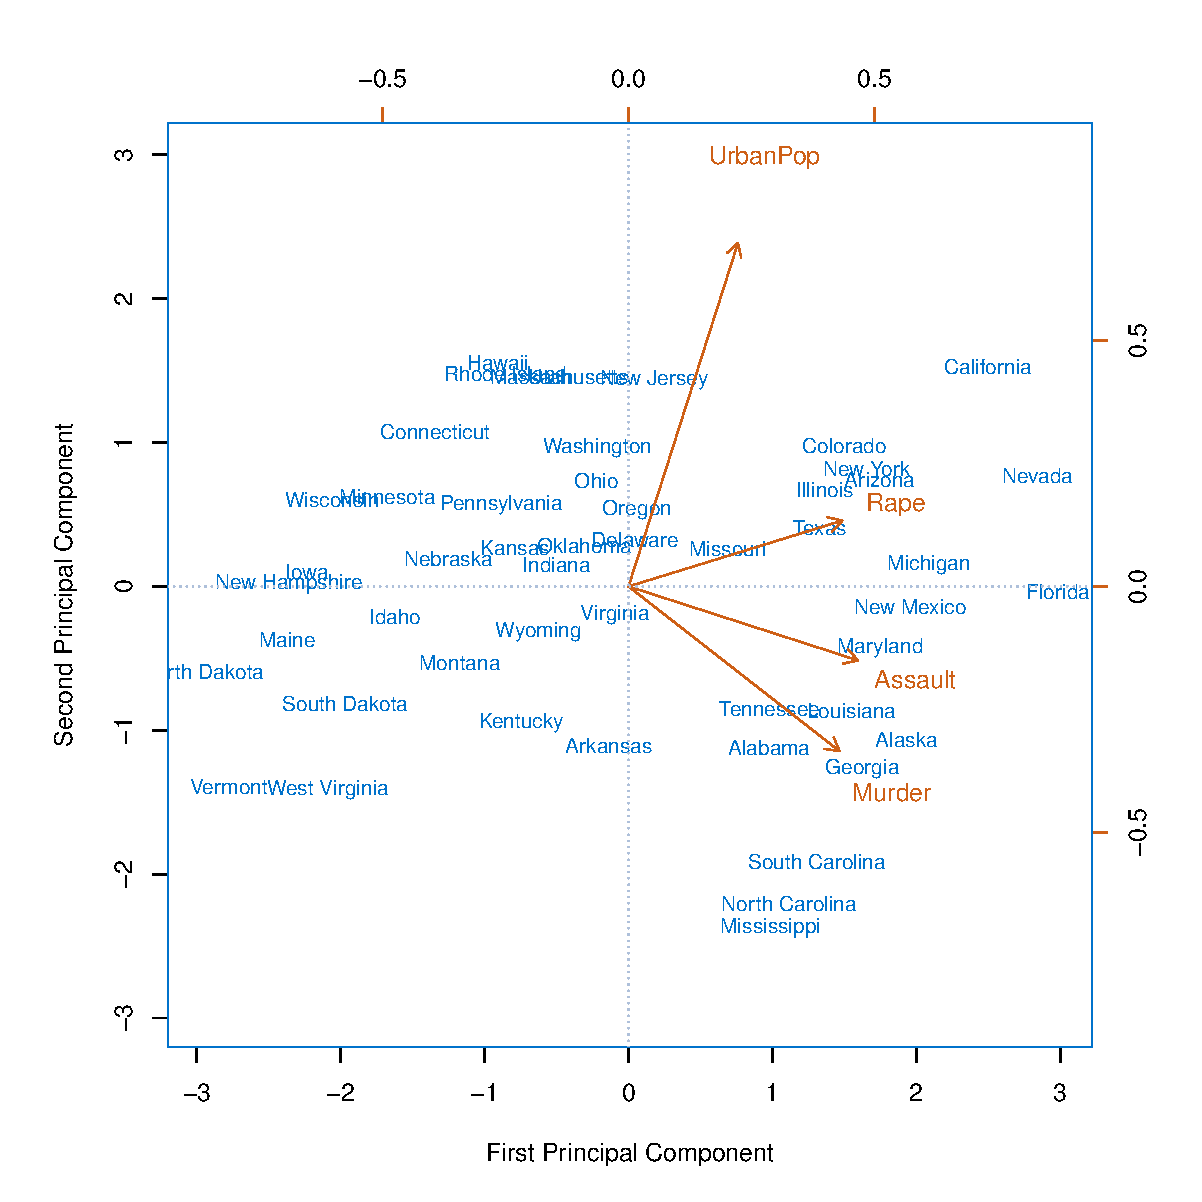
\includegraphics[width=.75\textwidth]{../class11/Figures_Chapters_7-13/Chapter12/12_1.pdf} \\

\scriptsize Source: ISLR2 Figure 12.1
\caption[US arrests data example -- Biplot]{US arrests data example -- Biplot with data plotted on first two principal components with original variables}
\label{fig:pca2}
\end{figure}

Interpretation of the principal components, which is important in explanation but less so in prediction, focuses on the loadings. For example, looking at the columns of the loadings in Table~\ref{tab:pca} shows that the first PC has high loadings on the variables ''Murder'', ''Assault'', and ''Rape'', and a much smaller loading on ''UrbanPop''. This suggests that PC1 expresses the overall prevalance of violent crime, as a summary of those three variables. In contrast, the second PC has a high loading on ''UrbanPop'', but a much lower (absolute) loading on the other three variables, indicating that it expresses primarily the one variable ''UrbanPop''. This interpretation is supported by Figure~\ref{fig:pca2}, which examines the rows of Table~\ref{tab:pca}, plotting each variable as a two-component vector in the space spanned by PC1 and PC2 (recall that the principal components are by definition orthogonal). Here, the row vector for the variable ''UrbanPop'' is visually distinct and separate from the row vectors for the other three variables. 

While the iterative description of principal components above illustrates the properties of the components in terms of their variance, actual PCA is done by means of \emph{eigendecomposition}. It turns out that the solution to the maximization problem in Equations~\ref{eq:pca1} and \ref{eq:pca2} are the principal components of the data correlation matrix. Each principal component is an \emph{eigenvector} of the data correlation matrix such that:

\begin{align*}
 V^{-1} X^T X V = V^{-1}CV = \Lambda
\end{align*}
\noindent where $V$ is the matrix whose columns are the \emph{eigenvectors}, $C$ is the data correlation matrix, and $\Lambda$ is a diagonal matrix of \emph{eigenvalues}.

\noindent The \emph{proportion of variance explained} $f_k$ by each PC $k$ is proportional to the corresponding \emph{eigenvalue} $\lambda_k$, that is, the k-th entry of $\Lambda$:
\begin{align*}
f_k = \frac{\lambda_k}{\sum_{j=1}^p \lambda_{j}} 
\end{align*}

\noindent The \emph{cumulative proportion of variance} $F_k$ explained by the first $k$ PC is then:
\begin{align*}
F_k = \frac{\sum_{j=1}^k \lambda_j}{\sum_{j=1}^p \lambda_{j}}
\end{align*}

There are different criteria for selecting the number of principal components to retain for further analyses:

\begin{itemize}
  \item There may be a theoretical reason, especially in an explanation context, to retain a specific number of principal components
  \item The analyst retains those principal components that have an intuitive and relevant interpretation, as in the above example. 
  \item The analyst retains those principal components whose eigenvalue $\lambda > 1$
  \item The analyst retains principal components until the cumulative proportion of variance explained by the components surpasses a given threshold, e.g. 80\%. For example, the right panel in Figure~\ref{fig:pca3} shows a plot of the cumulative variance explained. The first two principal components are necessary to explain 80\% or more of the total variance in the original data.
  \item When used in subsequent regression or classification models, cross-validation may be used to identify the optimal $K$ that shows the lowest test error.
  \item The analyst examines the ''\emph{scree plot}'', that is, the plot of the eigenvalues or proportion of variance explained by each component. Oftentimes, there will be a clear point of inflection in this plot, indicating a useful cutoff. The left panel in Figure~\ref{fig:pca3} shows such a scree plot. The proportion of variance explained diminishes for each additional principal component.
\end{itemize}

In practice, the number of principal components to retain is often subjective, and analysts use a combination of considerations and criteria to make their decision.

\begin{figure}
\centering
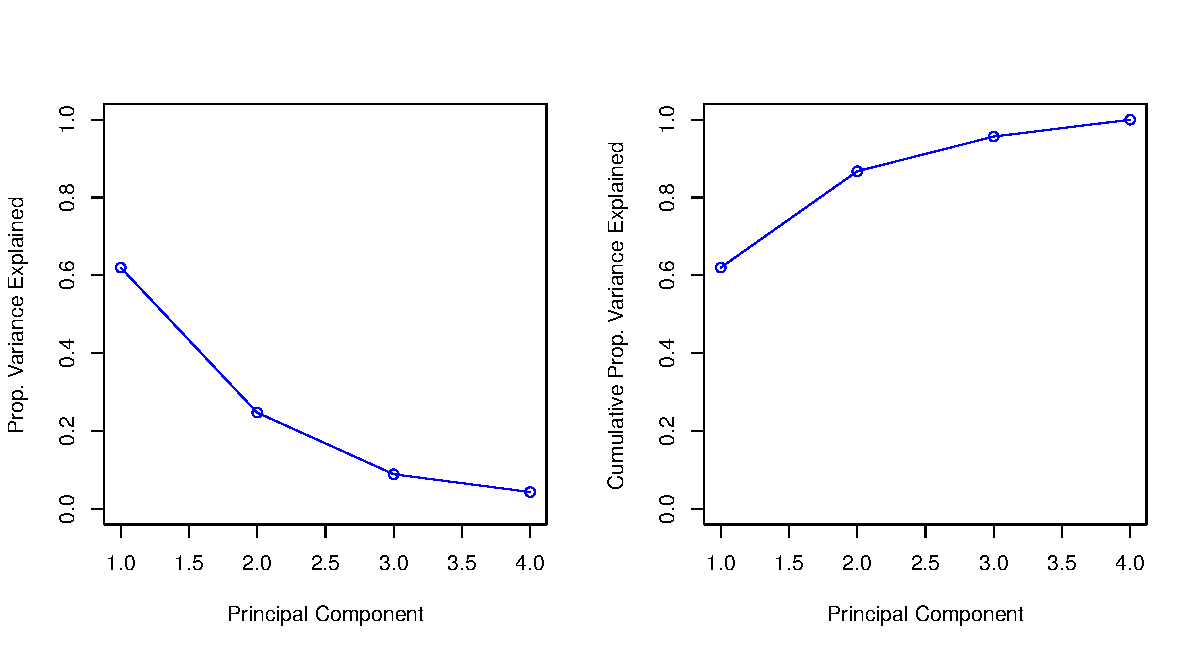
\includegraphics[width=.9\textwidth]{../class11/Figures_Chapters_7-13/Chapter12/12_3.pdf} \\

\scriptsize Source: ISLR2 Figure 12.3
\caption[US arrests data example -- Scree plot]{US arrests data example -- Scree plot and cumulative variance explained}
\label{fig:pca3}
\end{figure}

\section{Principal Components Analysis in R}

The \texttt{USArrests} in the \texttt{ISLR2} library contains data on the arrests (per 100,000 residents) for various violent crimes as well as the percentage of urban population in the 50 states of the US\footnote{The R code for this example is based on material in Section 12.5 of ISLR2}. First, examine the data and the correlation between variables. In the correlation matrix, one can already see that ''UrbanPop'' is not highly correlated with the other three variables, an indication that it will not load on the same principal component as those.

\begin{samepage}
\begin{Rcode}
library(ISLR2)
?USArrests
summary(USArrests)
cor(USArrests)
\end{Rcode}
\end{samepage}

\noindent The \texttt{prcomp()} function in R performs a PCA and can optionally scale and center the data before doing so:


\begin{samepage}
\begin{Rcode}
# PCA using prcomp()
# Scaling is generally a good idea
pca.result <- prcomp(USArrests, scale=TRUE)

# Print the component loadings
pca.result$rotation
\end{Rcode}
\end{samepage}

The results can be plotted in a biplot, similar to the one in Figure~\ref{fig:pca2}, using the \texttt{biplot()} function for the \texttt{prcomp} result object. By default, that function uses the first two principal components, but others can be specified using the \texttt{choices} argument. Note that the signs of the principal components may be arbitrarily flipped.

\begin{samepage}
\begin{Rcode}
# Biplot for components 1 and 2
biplot(pca.result, choices=1:2, scale=0)
\end{Rcode}
\end{samepage}

\noindent The explained variance can be computed from the result and plotted in a scree plot similar to the one in the left panel of Figure~\ref{fig:pca3}.

\begin{samepage}
\begin{Rcode}
# Explained variance for each component
pca.result$sdev^2

# Scree plot (both points and lines)
plot(pca.result$sdev^2, type='b', col='blue')
\end{Rcode}
\end{samepage}

\noindent Recall that the proportion of variance explained is the proportion of the variance of a principal component out of the total variance explained by all principal components. The R function \texttt{cumsum()} can be used to conveniently calculate the cumulative value of this. The following code block computes a cumulative plot similar to the right panel in Figure~\ref{fig:pca3}.

\begin{samepage}
\begin{Rcode}
# Proportion of variance explained
pve <- pca.result$sdev^2 / sum(pca.result$sdev^2)

# Cumulative sum of variance explained
plot(cumsum(pve), type='b', col='blue')
\end{Rcode}
\end{samepage}

\noindent Using the \texttt{eigen(.)} function for eigenvalue decomposion shows that the principal component loadings correspond to the eigenvectors and the explained variance corresponds to the eigenvalues, 

\begin{samepage}
\begin{Rcode}
# Eigen-decomposition of correlation matrix
e <- eigen(cor(USArrests))
# Compare values and vectors to prcomp results
e$values
e$vectors
\end{Rcode}
\end{samepage}


\noindent The component scores themselves are also available in the \texttt{prcomp} result for use in further analysis such as regression or classification:

\begin{samepage}
\begin{Rcode}
# Print the component scores themselves 
# For further use in regression, etc.
head(pca.result$x)
\end{Rcode}
\end{samepage}

\begin{tcolorbox}[colback=code]
\subsubsection*{Hands-On Exercise} 
The \texttt{Boston} dataset in the \texttt{ISLR2} library describes house prices in the different suburbs of Boston. Use PCA to reduce the number of dimensions for this dataset:
\begin{enumerate}
   \item Use the \texttt{prcomp} function to perform a PCA on the centered and standardized data. Limit yourself to quantitative inputs.
   \item Produce a biplot of the first two components
   \item Provide the proportion of variance explained by each component
   \item How many components would you retain? Why? How much of the total variance would this explain?
   \item Based on the loadings, can you ascribe meaning to the components? What do they represent?
\end{enumerate}
\end{tcolorbox}

\begin{tcolorbox}[colback=code]
\subsubsection*{Hands-On Exercise} 
The \texttt{Harmann74.cor} dataset in the \texttt{datasets} library contains the results of 24 psychological tests given to 145 school children. 
Use PCA to reduce the number of dimensions for this dataset:
\begin{enumerate}
   \item Use the \texttt{prcomp} function to perform a PCA on the centered and standardized data. Limit yourself to quantitative inputs.
   \item Produce a biplot of the first two components
   \item Provide the proportion of variance explained by each component
   \item How many components would you retain? Why? How much of the total variance would this explain?
   \item Based on the loadings, can you ascribe meaning to the components? What do they represent?
\end{enumerate}
\end{tcolorbox}

\begin{tcolorbox}[colback=code]
\subsubsection*{Hands-On Exercise} 
The \texttt{Hitters} dataset in the \texttt{ISLR2} library contains the salary of 322 baseball players and season statistics. Use \texttt{salary} as the target variable and all other numerical variables as predictors. 

\begin{enumerate}
   \item Use PCA to reduce the number of dimensions for the predictors. Limit yourself to quantitative inputs.
   \item Retain the first principal component.
   \item Estimate and cross-validate a regression model using the first PC as predictor. What is the training and validation error?
   \item Repeat steps (1) to (3), retaining 2, 3, \ldots, all components
   \item Plot the training and validation error agains the number of components. Describe and discuss your results.
\end{enumerate}
\end{tcolorbox}

\section{Clustering}

Whereas PCA tried to simplify a data set ''by column'' through the identification of variables that can be summarized by principal components, cluster analysis tries to simply a data set ''by row'' through the identification of observations that are similar and can be represented as a group, that is, a \emph{cluster}. The aim is to form homogenous subgroups of observations and to discover ''structure'' in the data.

There are a many different types of clustering. This chapter focuses on two simple and easy-to-understand methods. The \emph{k-means clustering algorithm} is an example of centroid-based clustering, a method that assigns observations to clusters based on their distance from the cluster center (''centroid''), while \emph{agglomerative clustering} is a form of hierarchical clustering which iteratively merges observations together to form larger and larger clusters. 

\subsection{K-Means Clustering}

In k-means clustering, the number of clusters $K$ is assumed given, determined by the analysts knowledge of the data or the requirements of the analysis. The aim of k-means clustering is to minimize the \emph{within-cluster variation} $W(C_i)$ in each cluster $C_i$:

\begin{align*}
\min_{C_i} \left\{ \sum_{k=1}^K W(C_k) \right\}
\end{align*}

\noindent This within-cluster variation is defined as the squared Euclidean distance between every pair of observations in the cluster (Equation~\ref{eq:cluster1}) or between every observation and the cluster \emph{centroid} of the cluster it is assigned to, that is, its corresponding cluster mean $\bar{\mu}$ (Equation~\ref{eq:cluster2}).

\begin{align}
W(C_k) &= \frac{1}{|C_k|} \sum_{i,i' \in C_k} \sum_{j=1}^p (x_{ij} - x_{i'j})^2 \label{eq:cluster1} \\
&= 2 \sum_{i \in C_k} \sum_{j=1}^p (x_{ij} - \bar{\mu}_{kj})^2 \label{eq:cluster2}
\end{align}

\noindent Here, $i, i'$ range over observations within cluster $C_k$, $j$ ranges over the $p$ different variables that make up an observation, and $\bar{\mu}_kj$ is the mean of variable $j$ for cluster $k$.

\begin{tcolorbox}[colback=alert]
\noindent This definition of distance means that k-means cluster analysis is only applicable to quantitative variables. 
\end{tcolorbox}

When variables are measured on different scales, e.g. one variables in the range of $[0, 1]$ while another is measured between $[0, 1000000]$ it is important to \emph{standardize or scale the variables to have similar standard deviations} (typically, unit standard deviation, i.e. 1). Otherwise, the Euclidean distance between observations is dominated by the variable with the largest range.

\begin{tcolorbox}[colback=alert]
Variables in the data set should be scaled to identical standard deviations prior to k-means clustering.
\end{tcolorbox}

\begin{figure}
\centering
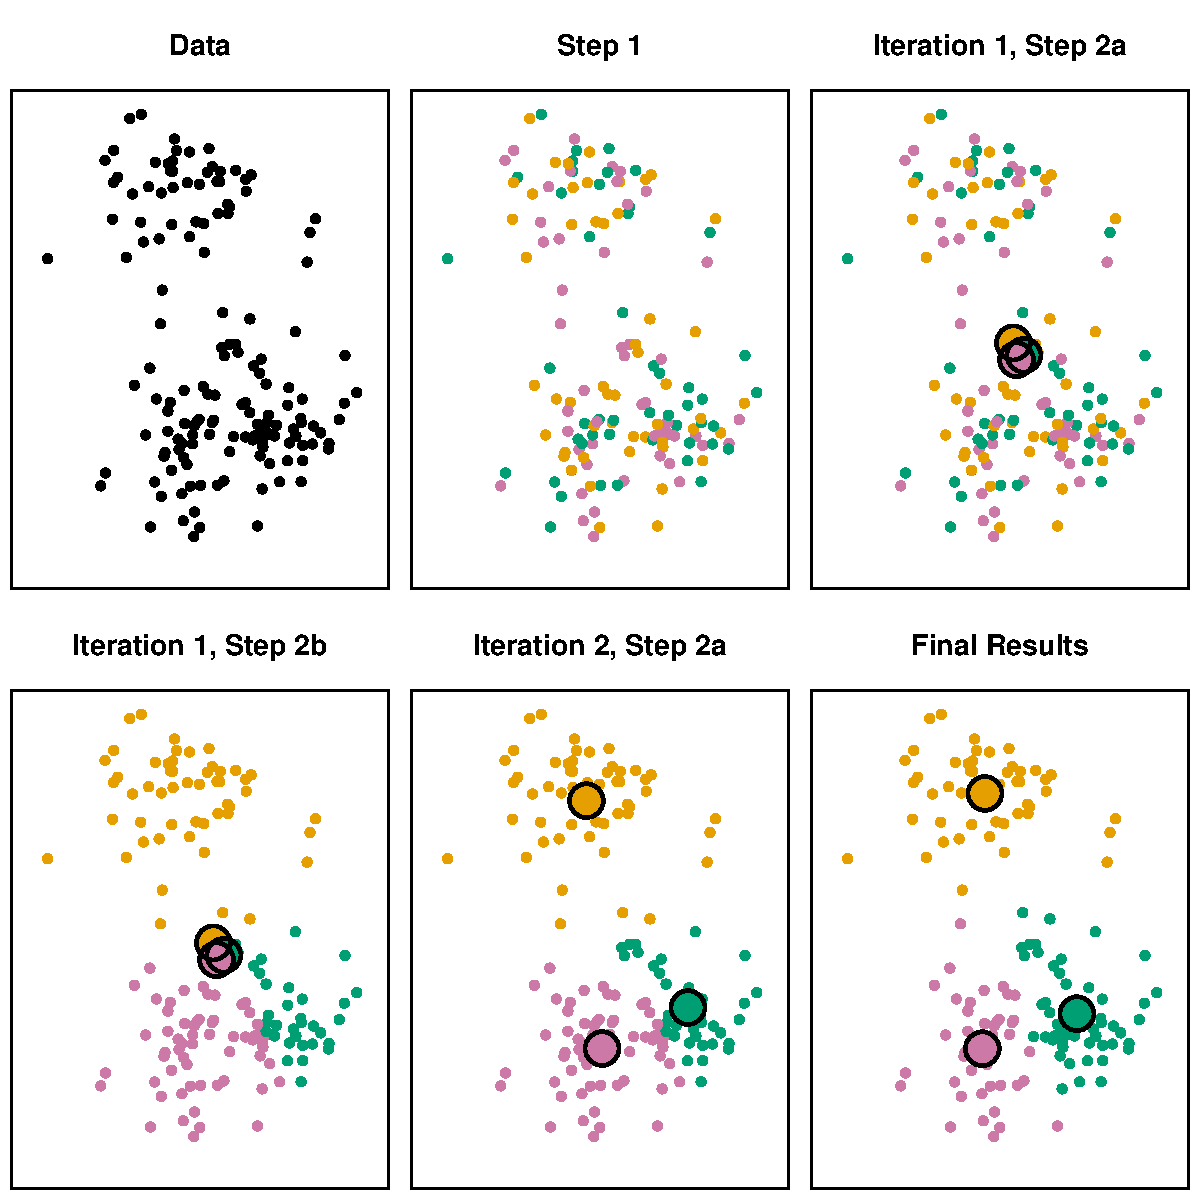
\includegraphics[width=.75\textwidth]{../class11/Figures_Chapters_7-13/Chapter12/12_8.pdf} \\

\scriptsize Source: ISLR2 Figure 12.8
\caption{K-means iterative cluster assignment example}
\label{fig:kmeans1}
\end{figure}

K-means clustering uses an iterative algorithm, beginning with the random assignment of each observation $i$ to one of the $k$ clusters. From these cluster assignments, the cluster means (centroids) can be computed ($\bar{\mu}_{kj}$ in Equation~\ref{eq:cluster2}). Next, each observation is assigned to that cluster whose centroid is closest. The last two steps are repeated until the cluster assignments no longer change. 

This process is illustrated in Figure~\ref{fig:kmeans1}. The top left panel shows observations on two variables. The panel labeled ''Step 1'' shows the initial random assignment of each observation to one of three clusters, indicated by the color. The top right panel, labelled ''Iteration 1, Step 2a'' shows the cluster means or centroids computed based on this assignment as large coloured circles. As one might imagine, random assignment leads to cluster means that are very similar. The bottom left panel, ''Iteration 1, Step 2b'' shows the cluster assignment of the observations based on the new cluster means. Each observation is assigned to that cluster whose mean is closest. The bottom middle panel, ''Iteration 2, Step 2a'' shows the new cluster means based on the new cluster assignment of observations. The bottom right panel shows the final, stable cluster assignment. Repeated calculation of cluster means and assigning observations to clusters does not change cluster membership for any observation. Note that the cluster membership in this final panel is slightly different than the one in the bottom middle panel, indicating at least one more iteration between the two panels. 

It should be clear from this description that the random initial cluster assignment has a significant impact on the final result. As the number of observations grow, the random effects generally diminish, but different random initial cluster assignments may yield different final clustering solutions. 

\begin{tcolorbox}[colback=alert]
\noindent The k-means algorithm should be run multiple times and the optimal solution, that is, the one with the lowest within-cluster variability, should be chosen for further analysis.
\end{tcolorbox}


\begin{figure}
\centering
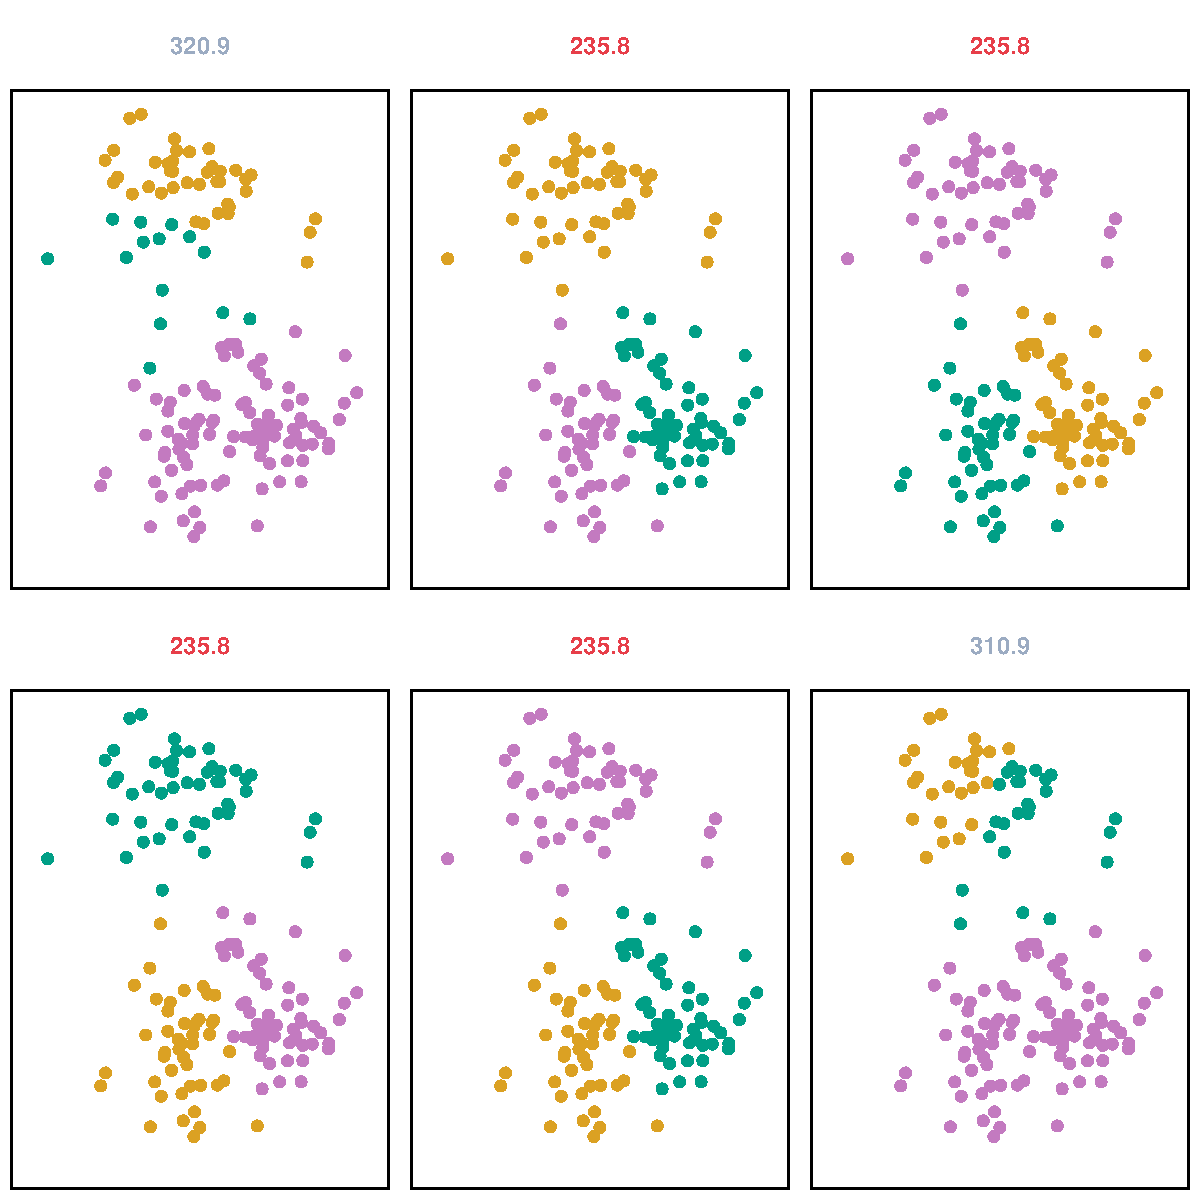
\includegraphics[width=.75\textwidth]{../class11/Figures_Chapters_7-13/Chapter12/12_9.pdf} \\

\scriptsize Source: ISLR2 Figure 12.9
\caption{K-means clustering solutions from different initial cluster assignments}
\label{fig:kmeans2}
\end{figure}

This effect is shown in Figure~\ref{fig:kmeans2}. The data from the previous example was clustered six different times with different random initial cluster assignments. Each final solution is different, and may also have a different \emph{within-cluster variability} as shown at the top of each panel. Note that some solutions are identical but permute the cluster assignments/colours. For example, the top middle and top right panels in Figure~\ref{fig:kmeans2} are identical and also identical with the bottom left and bottom middle solution, except for the permutation of cluster assignments, indicated by the colours. 

\subsection{K-Means Clustering in R}

To illustrate k-means clustering in R, consider the following simulated example, which uses the \texttt{kmeans()} function\footnote{The R code for this example is based on material in Section 12.5 of ISLR2}. Data is simulated as 50 observations on two normally distributed variables. One half of the data is shifted by $+3$ on the first variables and by $-4$ on the second variable. With a standard deviation of $1$, this constitutes a large separation and should lead to clearly identifiable clusters.

\begin{samepage}
\begin{Rcode}
# Set RNG seed for replicability
set.seed(2)
# Create a 50 x 2 matrix of random variables 
# Normally distributed, with 0 mean and SD=1
x <- matrix(rnorm(n=50*2, mean=0, sd=1), ncol=2)
# Clearly separate the first 25 points by shifting their coordinates
x[1:25, 1] <- x[1:25, 1] + 3
x[1:25, 2] <- x[1:25, 2] - 4
\end{Rcode}
\end{samepage}

\noindent Next, the data is clustered using the \texttt{kmeans()} function into 2 clusters, 20 times with different random initial cluster assignments:

\begin{samepage}
\begin{Rcode}
# Cluster into 2 clusters, performing 20 random starting assignments
km.result <- kmeans(x, 2, nstart=20)
\end{Rcode}
\end{samepage}

The result object \texttt{km.result} contains the cluster means, the cluster assignments for each observation and the sum-of-squares (distances) within each cluster and between clusters. Recall that the optimization objective is to minimize the within-cluster variation.

\begin{samepage}
\begin{Rcode}
# Results show cluster means, cluster assignments, 
# and sums of squares (distances) within and between 
print(km.result)
# Those values are also available as components in the result object
names(km.result)
print(km.result$centers)
print(km.result$withinss)
# etc.
\end{Rcode}
\end{samepage}

Finally, it is easy to create colour-coded plot of the data (the following R code block adds 1 to every cluster number to avoid plotting black points). This generates a plot as shown in Figure~\ref{fig:kmeans4}, clearly indicating the well-separated clusters.

\begin{samepage}
\begin{Rcode}
# Plot the color-coded points
plot(x, col=(km.result$cluster+1),
     main = 'K-Means Clustering Results with K=2',
     xlab = '', ylab='', pch=20, cex=2)
\end{Rcode}
\end{samepage}

\begin{figure}
\centering

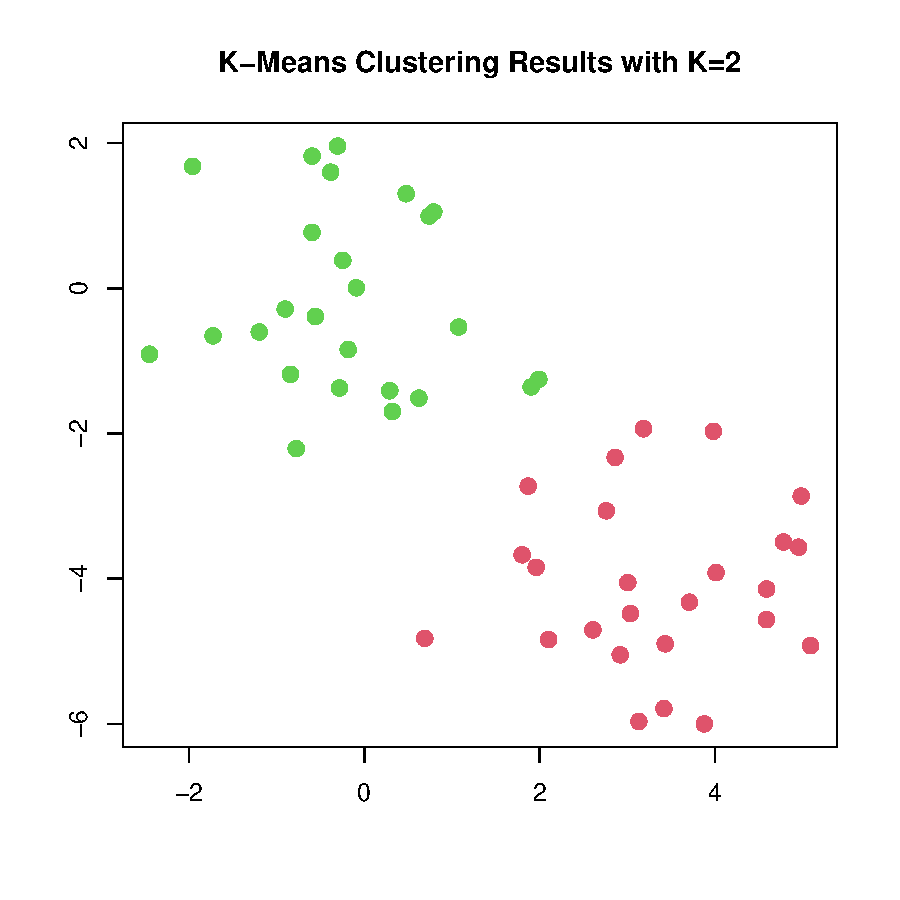
\includegraphics[height=3in]{kmeans.pdf}
\caption{Result of k-means clustering on simulated data}
\label{fig:kmeans4}
\end{figure}


\begin{tcolorbox}[colback=code]
\subsubsection*{Hands-On Exercise} 
The \texttt{Boston} dataset in the \texttt{ISLR2} library describes house prices in the different suburbs of Boston. Use K-Means Clustering to identify sets of similar suburbs using only the numerical variables in the data set.
\begin{enumerate}
   \item Use the \texttt{kmeans} function to perform a cluster analysis, using multiple starting assignments. Limit yourself to quantitative inputs but do not scale the variables.
   \item Use different numbers of clusters $k$ and identify which value of $k$ gives you the best results. Define what you mean by ''best'' and justify your choice.
   \item Scale the data so that each variable has the same variance or standard deviation, but do not change the variable means. 
   \item Repeat the cluster analysis with the best value of $k$ and compare results.\end{enumerate}
\end{tcolorbox}

\begin{tcolorbox}[colback=code]
\subsubsection*{Hands-On Exercise} 
The \texttt{Hitters} dataset in the \texttt{ISLR2} library contains the salary of 322 baseball players and season statistics. Use K-Means Clustering to identify sets of similar players, using only the numerical variables in the data set.

\begin{enumerate}
   \item Use the \texttt{kmeans} function to perform a cluster analysis, using multiple starting assignments. Limit yourself to quantitative inputs but do not scale the variable.
   \item Use different numbers of clusters $k$ and identify which value of $k$ gives you the best results. Define what you mean by ''best'' and justify your choice.
   \item Scale the data so that each variable has the same variance or standard deviation, but do not change the variable means. 
   \item Repeat the cluster analysis with the best value of $k$ and compare results.
\end{enumerate}
\end{tcolorbox}

\subsection{Hierarchical Clustering}

Hierarchical clustering is either \emph{agglomerative}, that is, it constructs clusters ''bottom-up'' by joining observations or small clusters to larger clusters, or it may be \emph{divisive}, that is, in ''top-down'' fashion, starting from the whole set of observations, it iteratively divides the set into clusters. This section examines the use of agglomerative clustering, which is widely used because of its intuitive process and its flexibility.

Agglomerative clustering begins with $n$ observations and a distance (or, alternatively, a similarity metric, which is just the inverse of distance -- a large distance means a small similarity). The process is then as follows:

\begin{enumerate}
   \item Treat each observation as its own cluster
   \item Repeat the following steps $n-2$ times:
   \begin{enumerate}
      \item Calculate distances between all pairs of clusters
      \item Identify the pair of clusters that are least distant from each other
      \item ''Fuse'' or merge these two clusters
   \end{enumerate}
\end{enumerate}

\begin{figure}
\centering
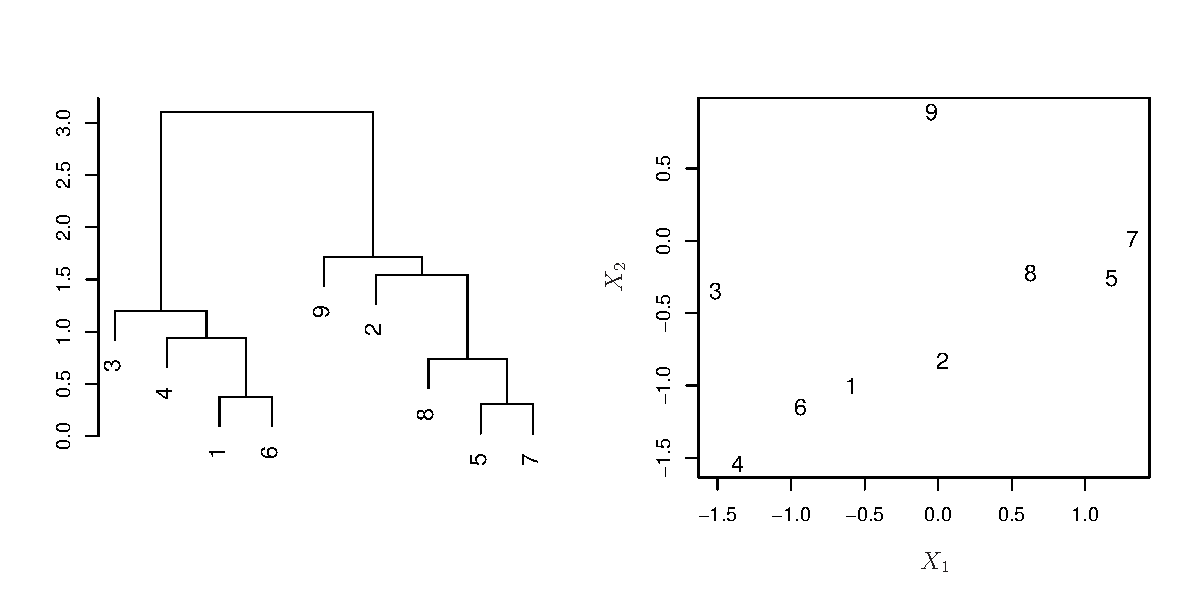
\includegraphics[width=.9\textwidth]{../class11/Figures_Chapters_7-13/Chapter12/12_12.pdf} \\

\scriptsize Source: ISLR2 Figure 12.12
\caption{Example dendrogram and data for agglomerative clustering}
\label{fig:dendro1}
\end{figure}

The process is usually visualized with a \emph{dendrogram}, which literally means ''tree graph'', such as the one shown in the left panel of in Figure~\ref{fig:dendro1}. A dendrogram is read bottom-up, showing which clusters are merged in which order. The vertical axis shows the distance between clusters as they are merged. Consider the observations on two variables shown in the right panel of Figure~\ref{fig:dendro1}. In the example, clusters 5 and 7 are merged first, from a distance of $\approx 0.3$. This distance is the smallest distance between all clusters, indicated as the lowest merging point in the dendrogram in the left panel of Figure~\ref{fig:dendro1}. Cluster 5 is just observation 5, and cluster 7 is just observation 7. The two together form a new cluster. Next, clusters 1 and 6 are merged, from a distance of $\approx 0.4$, the second lowest merging point in the dendrogram. Then, cluster 8 (which is observation 8) is added to the cluster consisting of observations 5 and 7, at a distance of $\approx 0.8$. After this, observation 4 is added to the cluster consisting of observations 1 and 6, etc. The final two clusters are at a distance of $\approx 3$ when they are merged into a single cluster. 

The follwing key decisions need to be made by the analyst for agglomerative clustering:

\begin{itemize}
   \item How to measure similarity or distance between observations?
   \item How to measure distance between clusters (''\emph{linkage}'')?
   \item How many clusters should there be?
\end{itemize}

Table~\ref{tab:distance} shows a set of common distance metrics or vector norms that are frequently used in agglomerative clustering. Figure~\ref{fig:distance} is a visualization of the intuition behind some of these distance metrics. For example, the Chebyshev distance allows diagonal ''moves'' to count as a single step with a distance of 1, wheres the taxicab metric counts a ''move'' in each direction as a single step, so that diagonal ''moves'' have a distance of 2. In principle, any of these distance metrics could also be used in k-means clustering, but this is rarely done.

Because the distance function is heavily influenced by the measurement scale of the variables, when these are not equal, it is possible for one variable to dominate others, simply because it is measured on a different scale. As with PCA and k-means clustering, it is therefore important to scale the variables in the data set to identical standard deviation (typically, unit standard deviation, i.e. 1). 

\begin{tcolorbox}[colback=alert]
Variables in the data set should be scaled to identical standard deviations prior to hierarchical clustering.
\end{tcolorbox}


\begin{table}
\renewcommand{\arraystretch}{2}
\centering 
\begin{tabular}{l|c|c} \hline
\begin{minipage}{1.75cm}Taxicab or Manhattan\end{minipage} & $ ||q-p||_1 $ & $\displaystyle \sum_i | q_i - p_i |$ \\ \hline
Euclidean & $ ||q-p||_2$ & $\displaystyle \sqrt{ \sum_i (q_i-p_i)^2}$ \\ \hline
Minkowski & $||q-p||_p$ & $\displaystyle \left( \sum_i | q_i - p_i |^p \right)^{\frac{1}{p}}$ \\ \hline
Chebyshev & $||q-p||_\infty$ & $\displaystyle \lim_{p \rightarrow \infty} \left( \sum_i | q_i - p_i |^p \right)^{\frac{1}{p}} = \max_i( | q_i - p_i | )$ \\ \hline
  & $||q-p||_{-\infty}$ & $\displaystyle \lim_{p \rightarrow -\infty} \left( \sum_i | q_i - p_i |^p \right)^{\frac{1}{p}} = \min_i( | q_i - p_i | )$ \\ \hline
\end{tabular}
\caption{Common distance metrics or ''norms'' in clustering}
\label{tab:distance}
\end{table}

\begin{figure}
\centering
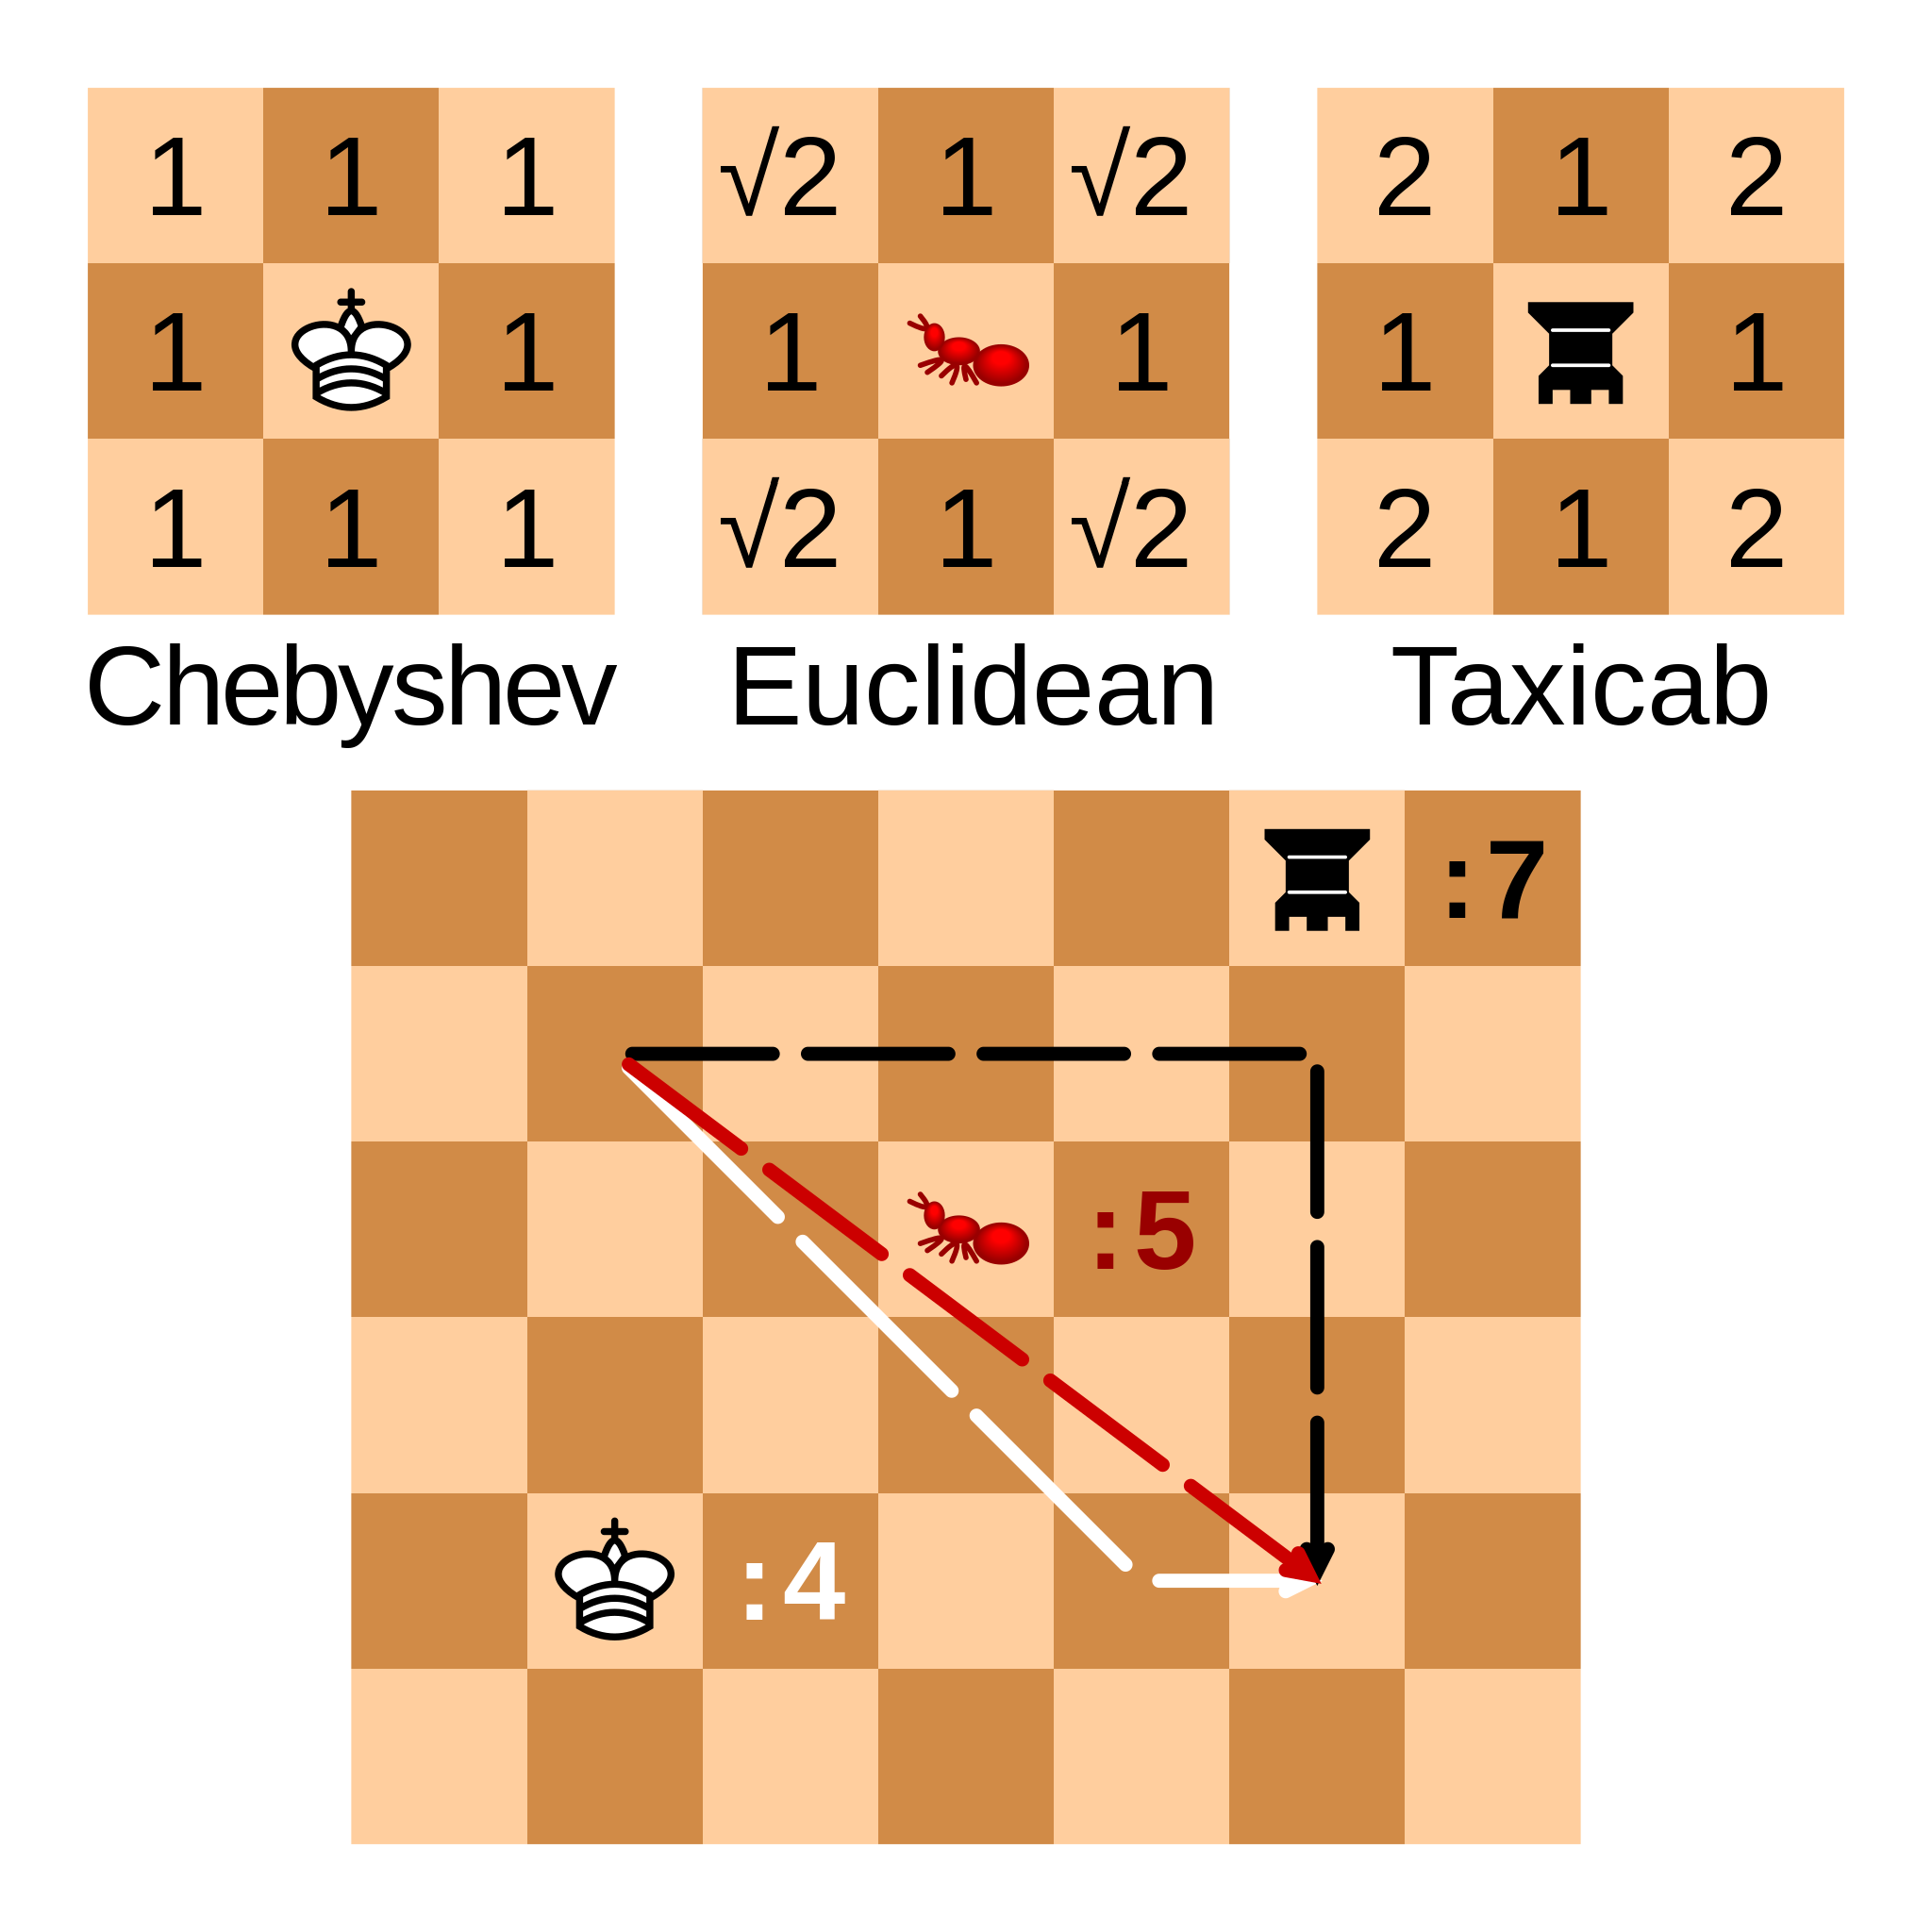
\includegraphics[height=3in]{Minkowski_distance_examples.svg.png} \\

\scriptsize \url{https://commons.wikimedia.org/wiki/File:Minkowski_distance_examples.svg}
\caption{Different distance metrics and their intuition}
\label{fig:distance}
\end{figure}

Table~\ref{tab:linkages} shows a set of the most commonly used \emph{linkage functions}, that is, functions that express the distance between two clusters $G$ and $H$. The \emph{single linkage} is based on the minimum distance of any pair of observations where one observation is in cluster $G$ and the other in cluster $H$. In other words, the distance of two clusters is the distance between the two closest observations from each cluster. In contrast, \emph{complete linkage} uses the maximum; the distance between clusters is the maximal distance between any of their member observations. Finally, \emph{average linkage} uses the mean distance between all pairs of observations. There are many other, less commonly used linkage functions available\footnote{\url{https://en.wikipedia.org/wiki/Hierarchical_clustering}}.

\begin{table}
\renewcommand{\arraystretch}{1.5}
\centering

\begin{tabular}{l|l} \hline
Single & $\displaystyle d_{SL}(G,H) = \min_{i \in G, i' \in H} d_{i, i'}$  \\ \hline
Complete & $\displaystyle d_{CL}(G,H) = \max_{i \in G, i' \in H} d_{i, i'}$  \\ \hline
Average & $\displaystyle d_{AL}(G,H) = \operatorname*{mean}_{i \in G, i' \in H} d_{i, i'}$  \\ \hline
\end{tabular}
\caption{Commonly used linkage functions in hierarchical clustering}
\label{tab:linkages}
\end{table}

The linkage function has a significant effect on the process of clustering a set of observations. Consider the three examples shown in the different panels of Figure~\ref{fig:dendro2}. Merging two observations into a cluster is always done at the same distance, as this is determined purely by the distance metric, not the linkage function. However, the decision which clusters (of multiple observations) to combine is heavily influenced by the linkage function as can be seen in the very different dendrograms in Figure~\ref{fig:dendro2}. 

\begin{figure}
\centering
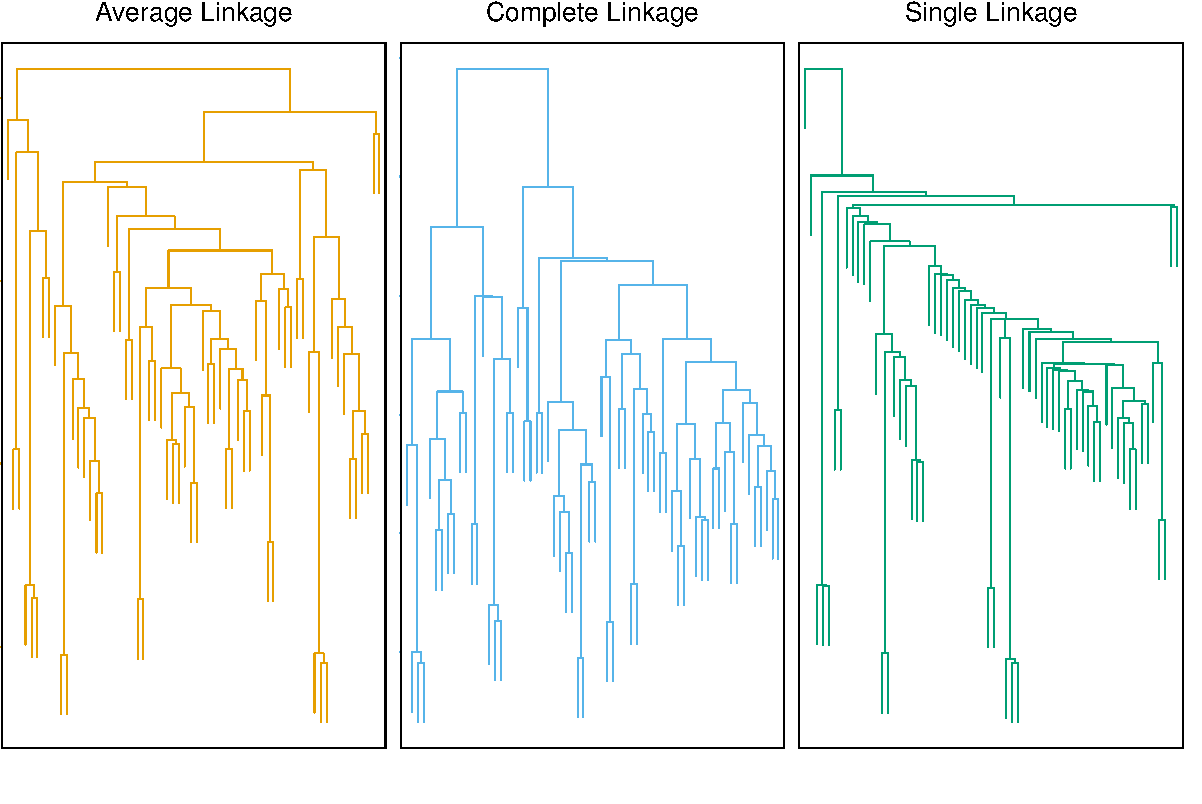
\includegraphics[width=.9\textwidth]{../class11/Figures_Chapters_7-13/Chapter12/12_14.pdf} \\

\scriptsize Source: ISLR2 Figure 12.14
\caption{The effect of different linkage functions in agglomerative clustering}
\label{fig:dendro2}
\end{figure}

The final question concerns the choice of the number of clusters. The answer to this question may be driven by theory (typically in explanatory applications), by requirements of the subsequent data analysis or the subsequent use of the resulting clusters, or by examining the distances at which clusters are merged, that is, the height in the dendrogram. Choosing a number of clusters is called ''cutting the dendrogram'' at a specific point. Consider the example in Figure~\ref{fig:dendro3}. The left panel shows the solution of the agglomerative clustering. In the end, a single cluster containing all the observations remains, with the last two clusters merged at a distance of $\approx 10.5$. The middle and right panel show two different ''cuts'' of the dendrogram, one resulting in two clusters and the other resulting in three clusters. The cuts may be determined by a desired number of clusters, by considerations of distance, or both. It should be clear that lowering the ''cut'' height further beyond what is shown in the right panel, that is reducing the distance between clusters, would result in many small clusters with a much smaller distance between them. 

\begin{figure}
\centering
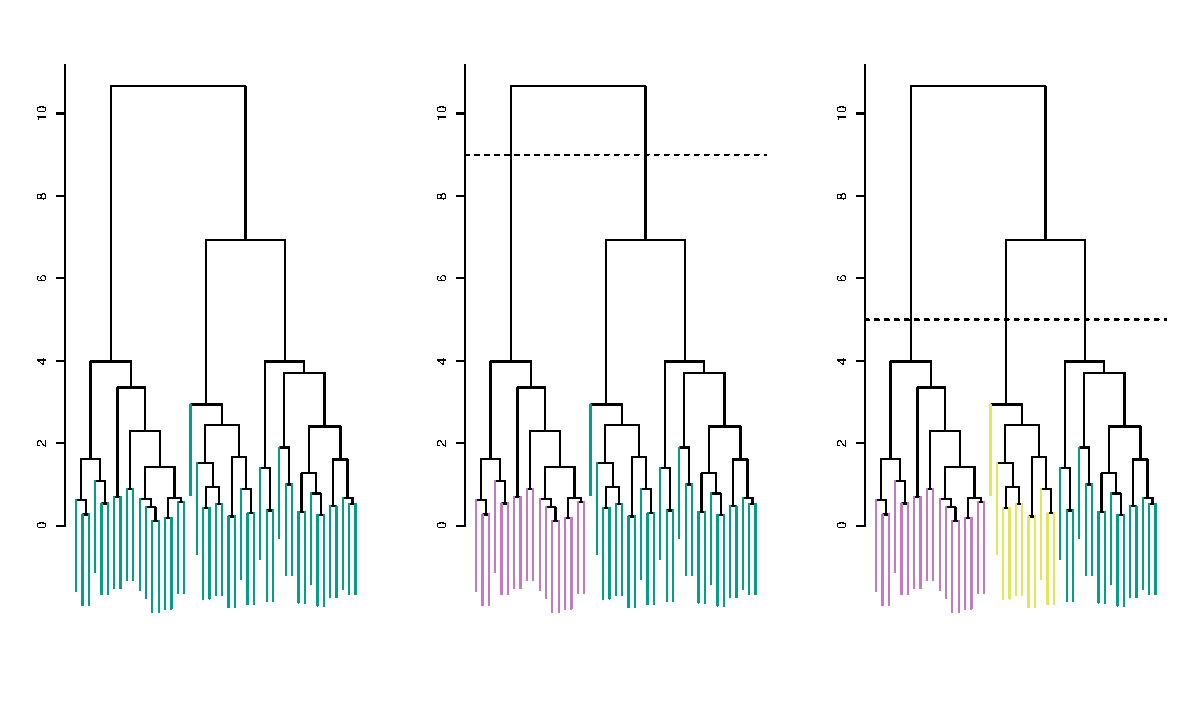
\includegraphics[width=\textwidth]{../class11/Figures_Chapters_7-13/Chapter12/12_11.pdf} \\

\scriptsize Source: ISLR2 Figure 12.11
\caption{Cutting a dendrogram to determine the number of clusters}
\label{fig:dendro3}
\end{figure}


\subsection{Hierarchical Clustering in R}

This example uses the same simulated data as the example for k-means clustering\footnote{The R code for this example is based on material in Section 12.5 of ISLR2}. First, generate 50 observations on two variables from a normal distribution. One half of the observations are shifted on both variables to provide a known cluster structure.

\begin{samepage}
\begin{Rcode}
# Set RNG seed for replicability
set.seed(2)
# Create a 50 x 2 matrix of random variables 
# Normally distributed, with 0 mean and SD=1
x <- matrix(rnorm(n=50*2, mean=0, sd=1), ncol=2)
# Clearly separate the first 25 points by shifting their coordinates
x[1:25, 1] <- x[1:25, 1] + 3
x[1:25, 2] <- x[1:25, 2] - 4
\end{Rcode}
\end{samepage}

The \texttt{dist()} function is used to calculate differences between the observations. The names for the \texttt{method} argument to \texttt{dist()} are the same as in Table~\ref{tab:distance}. Additionally, the \texttt{'maximum'} distance in R uses the greatest distance among all the variables of the two observations. 

\begin{samepage}
\begin{Rcode}
# The dist() function calculated distances
# according to a variety of metrics/norms
euclid.dist <- dist(x, method='euclidean')
pnorm.dist <- dist(x, method='minkowski', p=3)
manh.dist <- dist(x, method='manhattan')
max.dist <- dist(x, method='maximum')
\end{Rcode}
\end{samepage}

The \texttt{hclust()} function performs the hierarchical agglomerative clustering. The \texttt{method} argument specifies the type of linkage, according to Table~\ref{tab:linkages}. The \texttt{hclust()} function can use a few additional linkages not listed in that table, see the documentation (\texttt{?hclust}) for details. 

\begin{samepage}
\begin{Rcode}
# Use the hclust() function with a distance metric
hc.complete <- hclust(euclid.dist, method='complete')
hc.single <- hclust(euclid.dist, method='single')
hc.average <- hclust(euclid.dist, method='average')
\end{Rcode}
\end{samepage}

The dendrograms for the three different clustering solutions can be plotted to produce Figure~\ref{fig:dendro4}. 

\begin{samepage}
\begin{Rcode}
# Plot the dendrograms in a single plot
par(mfrow = c(1, 3))
plot(hc.complete , col='red', 
   main = "Complete Linkage", xlab = "", sub = "", cex = .9)
plot(hc.average , col='blue', 
   main = "Average Linkage", xlab = "", sub = "", cex = .9)
plot(hc.single , col='green', 
   main = "Single Linkage", xlab = "", sub = "", cex = .9)
\end{Rcode}
\end{samepage}

\begin{figure}
\centering
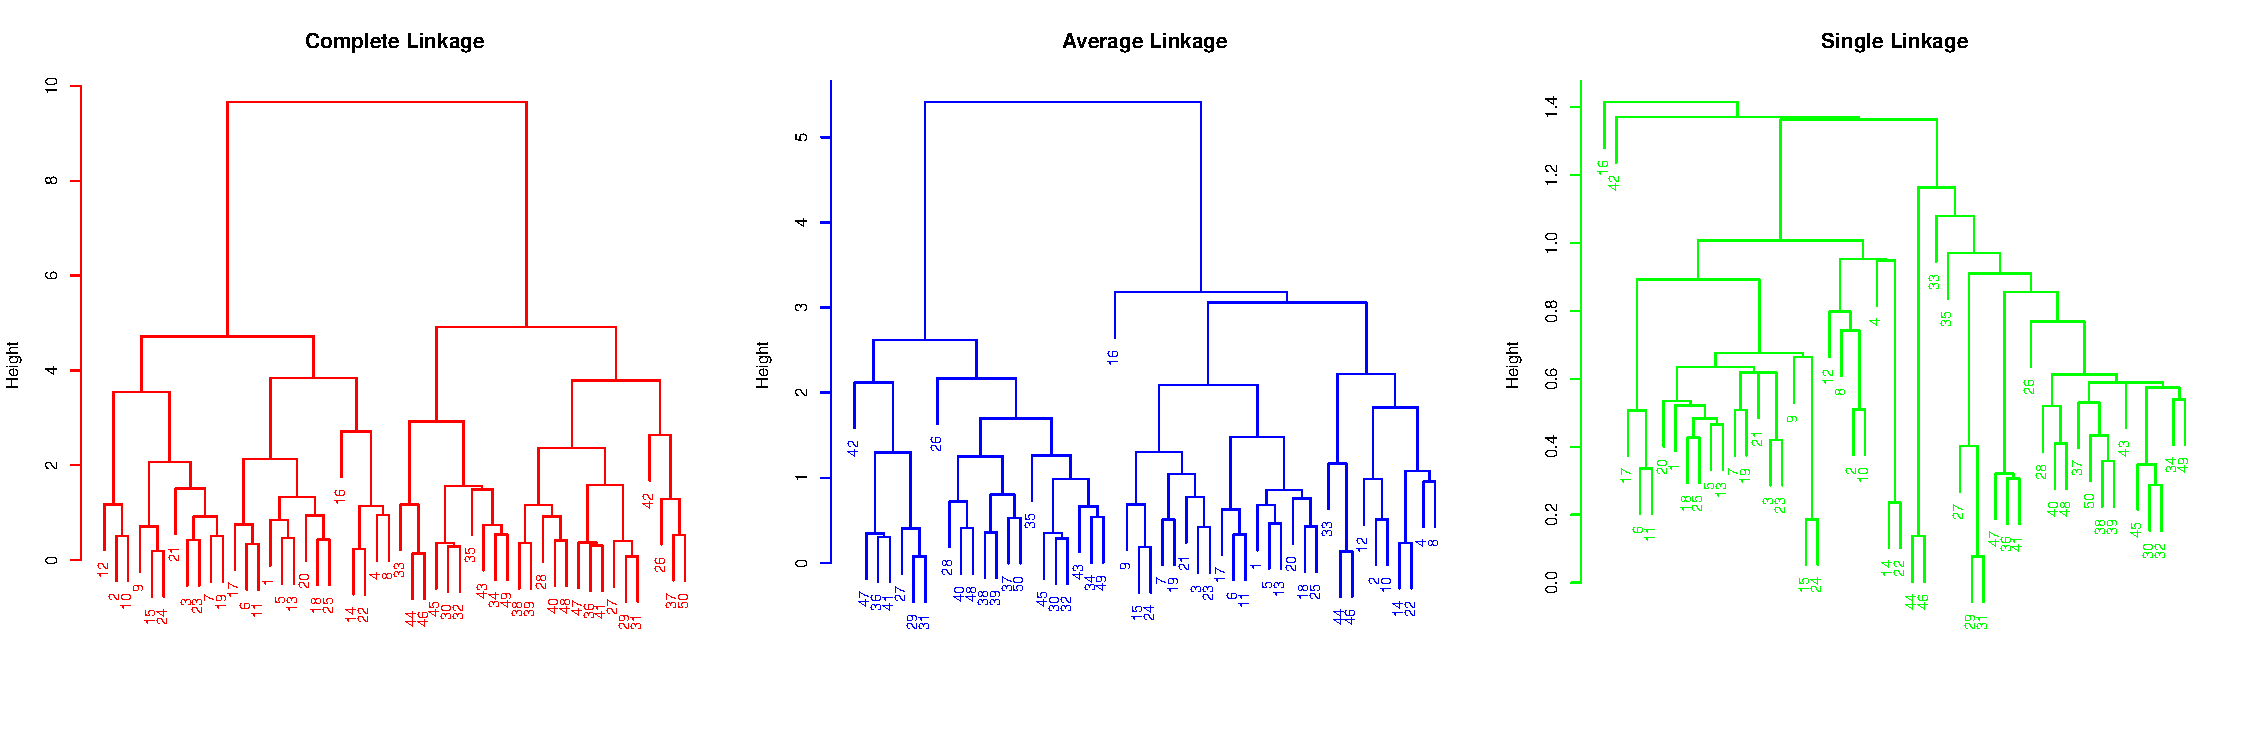
\includegraphics[width=\textwidth]{hclust.pdf}
\caption{Dendrogram of three clustering solutions for simulated data}
\label{fig:dendro4}
\end{figure}

The complete linkage and average linkage solutions are visually quite similar, but upon careful examination of which observations and clusters are merged in which order, they are actually very different from each other. The single linkage solution is visually very different from the others. Note the ''height'' of the dendrogram on the vertical axis. Because the single linkage focuses on the minimal distance between a pair of observations from each cluster, the heights in this dendrogram are the smallest among the three dendrograms. Because the average linkage focuses on the mean of distances of pairs of observations of two clusters, its height values are generally larger, but still smaller than the range of heights for the complete linkage solution, which focuses on the maximum distance between pairs of observations from two clusters. 

Finally, cutting the dendrogram is done with the \texttt{cutree()} function by specifying either the number of clusters $k$ or the height $h$ at which the dendrogram is to be cut. The function returns a vector with the cluster membership for each observation.

\begin{samepage}
\begin{Rcode}
# Cut by number of groups/clusters
cutree(hc.complete, k=4)
# Cut by height (distance)
cutree(hc.complete, h=6)
\end{Rcode}
\end{samepage}

\begin{tcolorbox}[colback=code]
\subsubsection*{Hands-On Exercise} 
The \texttt{Boston} dataset in the \texttt{ISLR2} library describes house prices in the different suburbs of Boston. Use Hierarchical Clustering to identify sets of similar suburbs using only the numerical variables in the data set.
\begin{enumerate}
   \item Use the \texttt{hclust} function to perform a cluster analysis, exploring different distance metrics and linkage functions. Limit yourself to quantitative inputs.
   \item Examine the dendrograms and identify which combination of distance metric and linkage function gives you the ''best'' solution. Define ''best'' and justify your decision.
   \item How many clusters $k$ would you choose?
   \item Using this value for $k$, perform a k-means Clustering and compare the results. Remember that k-means clustering uses the Euclidean distance.
\end{enumerate}
\end{tcolorbox}

\begin{tcolorbox}[colback=code]
\subsubsection*{Hands-On Exercise} 
The \texttt{Hitters} dataset in the \texttt{ISLR2} library contains the salary of 322 baseball players and season statistics. Use Hierarchical Clustering to identify sets of similar players, using only the numerical variables in the data set.

\begin{enumerate}
   \item Use the \texttt{hclust} function to perform a cluster analysis, exploring different distance metrics and linkage functions. Limit yourself to quantitative inputs and make sure you scale the data.
   \item Examine the dendrograms and identify which combination of distance metric and linkage function gives you the ''best'' solution. Define ''best'' and justify your decision.
   \item How many clusters $k$ would you choose?
   \item Using this value for $k$, perform a k-means clustering and compare the results. Remember that k-means clustering uses the Euclidean distance.
\end{enumerate}
\end{tcolorbox}

\begin{tcolorbox}[colback=code]
\subsubsection*{Hands-On Exercise} 
The \texttt{Auto} dataset in the \texttt{ISLR2} library contains information on 392 vehicles. Use Hierarchical Clustering to identify sets of similar vehicles, using only the numerical variables in the data set.

\begin{enumerate}
   \item Use the \texttt{hclust} function to perform a cluster analysis, exploring different distance metrics and linkage functions. Limit yourself to quantitative inputs.
   \item Examine the dendrograms and identify which combination of distance metric and linkage function gives you the ''best'' solution. Define ''best'' and justify your decision.
   \item How many clusters $k$ would you choose?
   \item Using this value for $k$, perform a k-means Clustering and compare the results. Remember that k-means clustering uses the Euclidean distance.
\end{enumerate}
\end{tcolorbox}

\section{Review Questions}

\paragraph*{Principal Components Analysis}

\begin{enumerate}[nosep]
    \item Explain how unsupervised machine learning differs from supervised machine learning in terms of data requirements and outcomes.
    \item What are the main goals of Principal Component Analysis (PCA) in data analysis?
    \item Explain the concept of "variance" in the context of PCA. Why is maximizing variance an important objective?
    \item How can PCA be used to simplify a complex dataset? Give an example based on a hypothetical dataset.
    \item How can PCA contribute to improving the interpretability of complex models?
    \item Describe the process of calculating the first principal component in PCA. What role do the loading vectors play? What optimization problem does PCA solve?
    \item How does one interpret the loadings of a principal component and what do they signify about the variables involved?
    \item Discuss the importance of scaling input variables before performing PCA. What could potentially happen if the variables are not scaled?
    \item Describe the relationship between eigenvalues and the variance explained by the principal components. How does one interpret these eigenvalues in practical terms?
    \item Provide several criteria that could be used to decide how many principal components to retain in an analysis.
    \item Discuss the relevance of the ''scree plot'' in determining the number of principal components to retain. What does an inflection point in the scree plot typically indicate?
    \item Explain how the biplot can be used to visualize both the principal components and the original variables. What insights can one gain from such a visualization?
    \item Explain how PCA can be used as a feature extraction technique in machine learning models.
\end{enumerate}
\paragraph*{K-Means Clustering}
\begin{enumerate}[nosep,resume*]
    \item Define clustering in the context of unsupervised machine learning and explain its main purpose.
    \item Compare and contrast the goals of principal component analysis (PCA) and clustering.
    \item What are centroid-based clustering and hierarchical clustering? Provide examples of each.
    \item Describe the k-means clustering algorithm. What objective does it aim to achieve?
    \item Explain the concept of within-cluster variation in the context of k-means clustering.
    \item What are the implications of variable scales on the performance of the k-means clustering algorithm? Why might scaling be necessary?
    \item Illustrate the iterative process of the k-means clustering algorithm. What happens in each step?
    \item Explain why the initial random assignment of observations to clusters can affect the final clustering solution in k-means.
    \item Discuss the importance of running the k-means algorithm multiple times. How does this practice influence the reliability of the clustering results?
    \item What are the computational complexities of k-means and hierarchical clustering? How do these affect their scalability to large datasets?
    \item Discuss the limitations of k-means clustering and possible scenarios where it might not perform well.
\end{enumerate}
\paragraph*{Hierarchical Clustering}
\begin{enumerate}[nosep,resume*]
    \item Describe a scenario in which hierarchical clustering would be more beneficial than k-means clustering. Consider aspects such as data structure and analysis goals.
    \item Describe hierarchical clustering and differentiate between agglomerative and divisive clustering.
    \item Explain the initial steps in an agglomerative clustering process. How does it begin, and what happens in the initial stages?
    \item Define a dendrogram and explain how it is used in hierarchical clustering.
    \item Discuss the significance of distance measures in hierarchical clustering. How do they affect the clustering process?
    \item How might the concept of distance be adapted when clustering categorical data using hierarchical methods?
    \item What are the different types of linkage methods in hierarchical clustering? Describe at least three and explain how they influence the clustering results.
    \item Provide an overview of common distance metrics used in agglomerative clustering. How might the choice of distance metric influence the outcome of clustering?
    \item Explain the process of creating a dendrogram and interpreting its structure in the context of hierarchical clustering.
    \item Explore the relationship between the number of observations and the interpretability of the dendrogram in hierarchical clustering. How does increasing the number of observations affect the clarity and usefulness of the dendrogram?
    \item Explain the concept of ''cutting the tree'' in hierarchical clustering. How does this process determine the number of clusters?
    \item Discuss how the choice of linkage method might impact the sensitivity of hierarchical clustering to outliers and noise in the dataset.
    \item How does the analyst decide on the number of clusters in hierarchical clustering? What factors might influence this decision?
    \item Consider the distance metrics shown in Table~\ref{tab:distance}. Which metric would be most appropriate for clustering data with extreme outliers and why?
    \item Explain why it might be necessary to standardize variables before performing hierarchical clustering.
    \item Evaluate the computational complexity of hierarchical clustering. How does this complexity influence the scalability of the method to large datasets?
\end{enumerate}
